\documentclass{article}

\usepackage[margin=1in]{geometry}
\usepackage{amsmath,amsthm,amssymb}
\usepackage{bbm,enumerate,mathtools}
\usepackage[hidelinks]{hyperref}
\usepackage{biblatex}
\addbibresource{geodesic.bib}
\usepackage{tikz}
\usetikzlibrary{arrows}

\newcommand{\fn}[3]{#1 \colon #2 \rightarrow #3}
\newcommand{\set}[1]{\left\{#1\right\}}
\newcommand{\ang}[1]{\left\langle#1\right\rangle}
\newcommand{\pd}[2]{\frac{\partial #1}{\partial #2}}

\theoremstyle{definition}
\newtheorem{definition}{Definition}[section]

% \theoremstyle{example}
\newtheorem{example}{Example}[section]

% \theoremstyle{conjecture}
\newtheorem{conjecture}{Conjecture}[section]

\theoremstyle{remark}
\newtheorem{remark}{Note}[section]

\newtheorem{theorem}{Theorem}[section]

\begin{document}

\title{Closed Geodesics: Topological Existence Theorems}
\author{Peter Kagey}

\maketitle
% How do we measure the length of a curve?

% Definition of geodesic
A note to begin: I wrote this paper with a particular audience in mind, namely
me in February of this year. I tried to capture a few things: (1) intuition for
the topic (2) rigorous definitions, (3) early theorems and consequences,
(4) modern theorems, and (5) conjectures and open problems.

\begin{section}{Preliminaries}
  The intuition in this paper is to think of a creature who lives in a manifold
  walking in a ``straight'' line in some sense at a constant
  (nonzero) speed. In particular, some examples worth keeping in mind are \begin{itemize}
    \item the torus $\mathbb R^2/\mathbb Z^2$, where ``straight lines'' are inherited from $\mathbb R^2$;
    \item the round sphere $\set{(x, y, z) \in \mathbb R^3 : x^2 + y^2 + z^2 = 1} = S^2 \subset \mathbb R^3$, where ``straight lines'' are great circles;
    \item a very ``wobbly'' sphere embedded in $R^3$; and
    \item $\mathbb R^3 \setminus \set{0}$, where straight lines are ordinary lines in $\mathbb R^3 \setminus \set 0$,
  \end{itemize}
  where the last example is included to avoid the dangers of thinking about only
  so-called ``geodesically complete'' $2$-manifolds.

  In the case of $\mathbb R^n$, the notion of acceleration along a path at
  some point in time follows from the usual calculus definition, since the
  notion of subtracting
  velocity vectors at two different points along the curve can be done naively,
  allowing the second derivative computation to work in the expected way \[
    \gamma''(t) = \lim_{h \rightarrow 0} \frac{\gamma'(t + h) - \gamma'(t)}{h}.
  \] However, one has to be careful when talking about acceleration
  in a general manifold. In particular, $T_{\gamma(t)}$ and $T_{\gamma(t+h)}$ are
  generally different tangent spaces, and the notion of subtracting such velocity
  vectors is decidedly more subtle. In particular, an isometric embedding of a
  Riemannian manifold into Euclidean space via $\fn f M {\mathbb R^n}$,
  preserves notions of velocity, but ``zero acceleration'' curves in the sense of
  geodesics may not be ``zero acceleration'' in an extrinsic sense
  (for example, a constant speed particle moving along $S^1 \subset \mathbb R^2$
  accelerates toward the origin.)
  We can fix this by considering the projection of the acceleration to the
  tangent plane, but capturing an \textit{intrinsic} notion of a directional
  derivative is more subtle.
  % Note: geodesics satisfy the properties of (non-euclidean) geometry
  % In this section, $M$ will always refer to a connected smooth manifold with or
  % without boundary unless otherwise noted, and $\nabla$ will refer to a connection in
  % $TM$.
  \begin{definition}
    Let $\fn \pi E M$ be a smooth vector bundle over $M$. Then a \textbf{connection} in
    $E$ is any map that sends a tangent vector field and a section of $E$ to
    another section of $E$ \[
      \fn{\nabla}{\mathfrak X(M) \times \Gamma(E)}{\Gamma(E)}
    \] denoted $\nabla_XY := \nabla(X, Y)$ and satisfying the following three properties:
    \begin{enumerate}[(i)]
      \item $\nabla$ is $C^\infty(M)$-linear in the first argument:
        $\displaystyle\nabla_{f_1X_1 + f_2X_2}Y = f_1\nabla_{X_1}Y + f_2\nabla_{X_2}Y$
      \item $\nabla$ is $\mathbb R$-linear in the second argument:
        $\displaystyle\nabla_X(a_1Y_1 + a_2Y_2) = a_1\nabla_X Y_1 + a_2\nabla_XY_2$, and
      \item $\nabla$ satisfies a product rule in the second argument:
        $\displaystyle\nabla_X(fY) = f\nabla_{X}Y + \underbrace{(Xf)}_{\in C^\infty(M)}Y$.
    \end{enumerate}
    % Connections are generalizations of directional derivatives with respect to
    % $X$, a tangent vector field.
  \end{definition}
  \begin{remark} % https://youtu.be/nEaiZBbCVtI
    In the case where $\Gamma(E) = C^\infty(M)$, $\nabla(X, f) := Xf$ satisfies
    the above properties. In particular, $\nabla$ can be thought of as a
    prescription for extending $\fn X {C^\infty(M)}{C^\infty(M)}$ to act on other
    vector bundles.
  \end{remark}
  \begin{example}
    Consider the case of $M = \mathbb R^3$ with the section of the tangent
    bundle given by  $\ang{x, 1, e^y} = X \in \mathfrak X(\mathbb R^3)$
    and a section of a rank-2 vector bundle $\ang{x^2, y + z} = Y \in \Gamma(E)$. Then taking
    the derivative of $Y$ along $X$ yields \[
      \nabla_XY = \underbrace{\begin{bmatrix}
        \displaystyle\pd{x^2}{x} & \displaystyle\pd{x^2}{y} & \displaystyle\pd{x^2}{z} \\
        \\
        \displaystyle\pd{(y+z)}{x} & \displaystyle\pd{(y + z)}{y} & \displaystyle\pd{(y + z)}{z}
      \end{bmatrix}}_{dY(x,y,z)}
      \underbrace{\begin{bmatrix}
        x \\~\\ 1 \\~\\ e^y
      \end{bmatrix}}_{X} =
      \underbrace{
        \begin{bmatrix}
          2x^2 \\~\\ 1 + e^y
        \end{bmatrix}
      }_{\in \Gamma(E)}.
    \] The matrix multiplication perspective makes it clearer to see that in
    this case (i) $\nabla$ is $C^\infty(\mathbb R^3)$-linear in the first
    term, because the column vector is $C^\infty(\mathbb R^3)$-linear,
    (ii) $\nabla$ is $\mathbb R$-linear in the second term because both partial
    derivatives and matrices are $\mathbb R$-linear, and (iii) holds by doing
    the product rule entrywise in the Jacobian matrix $d(fY)(x,y,z)$.
  \end{example}
  These conditions capture, in some sense, the ``essential qualities'' of
  taking the directional derivative of a vector bundle over a given section of
  the tangent bundle.
  \begin{remark}
    When on a Riemannian manifold, it is common to use a particular connection
    called the Levi-Civita connection, which is compatible with the metric in
    the expected way, and which has some other nice properties.
  \end{remark}
  \begin{definition}
    The \textbf{Levi-Civita connection} is a connection
    \[
      \fn\nabla {\mathfrak X(M) \times \mathfrak X(M)} {\mathfrak X(M)}
    \] such that for any tangent vector fields $X, Y \in \mathfrak X(M)$,
    $\nabla$ is
    \begin{enumerate}[(a)]
      \item compatible with the metric: $\nabla_X(g(Y, Z)) = g(\nabla_XY, Z) + g(Y, \nabla_XZ)$, and
        % the metric is preserved under $\nabla$, that is, $\nabla_{\!(-)\,}g \equiv 0$, and
      \item torsion-free: $\nabla_XY - \nabla_YX = [X, Y]$.
    \end{enumerate}
  \end{definition}
  \begin{remark}
    When the Levi-Civita connection exists, it is unique.
  \end{remark}
  \begin{remark}
    The second condition gets its name from the definition of the torsion,
    namely \[
      T(X, Y):= \nabla_XY - \nabla_YX - [X, Y].
    \]
    % What is torsion on a 2-manifold? Always 0?
  %   The inner product $g$ on the tangent bundle is a vector space, and
  %   so the action of $\nabla$ on $g$ is well-defined.
  \end{remark}
  % Being able to take the derivative of a section of a vector bundle in the
  % direction of the tangent bundle is the first step to being able to take the
  \begin{definition}
    Let $\nabla$ be a connection in tangent bundle $TM$, and let $\gamma$ be a
    curve in $M$. Then the \textbf{covariant derivative along} $\boldsymbol{\gamma}$ is the
    (unique) map $
      \fn {D_\gamma }{\mathfrak X(\gamma)}{\mathfrak X(\gamma)}
    $ satisfying the following three properties \begin{enumerate}[(i)]
      \item $\displaystyle D_\gamma (aV + bW) = aD_\gamma V + bD_\gamma W$
      \item $\displaystyle D_\gamma (fV) = f'V + fD_\gamma V$
      \item $\displaystyle D_\gamma V(t) = \nabla_{\gamma'(t)}\widetilde{V}$ for every extension $\widetilde V$ of $V$.
    \end{enumerate}
  \end{definition}
  \begin{remark}
    This definition is sensible, because (i) and (ii) respectively correspond to
    (ii) and (iii) in the definition of a connection, and the last condition is
    roughly says that the derivative along $\gamma$ should agree with a
    restriction on a vector field which is equal to $\gamma'$ along the curve.
  \end{remark}
  \begin{definition}
   For every smooth map from an interval to the manifold, $\fn \gamma I M$,
   define the \textbf{acceleration of $\gamma$} as the vector field
   $D_\gamma  \gamma'$ along $\gamma$.
  \end{definition}

  \begin{definition}
    A smooth curve $\gamma$ is called a \textbf{geodesic} (with respect to
    $\nabla$) if it's acceleration is zero: $D_\gamma \gamma' \equiv 0$.
  \end{definition}

  % \begin{figure}
  %   \begin{tikzpicture}
  %   % Example of a geodesic or two.
  %   % Poincare disk?
  %   \end{tikzpicture}
  % \end{figure}

  \begin{theorem}[Existence and uniqueness of geodesics; from \cite{Lee}, Theorem 4.27] % Lee Theorem 4.27
    Let $M$ be a smooth manifold and $\nabla$ a connection. Then for every
    $p \in M$ and $v \in T_pM$ there exists an interval $I \subset \mathbb R$
    around $0$ and a geodesic
    $\fn \gamma I M$ satisfying $\gamma(0) = p$ and $\gamma'(0) = v$.

    Furthermore, any two geodesics with the same initial conditions agree on
    their common domain.
  \end{theorem}
  \begin{proof}[Proof idea]
    The proof of the theorem works by moving to local coordinates in a way that respects
    the connection, and then making an appeal to uniqueness and existence for
    (second order) ordinary differential equations.
  \end{proof}

  \begin{definition}
    Given a geodesic $\fn \gamma I M$, an
    \textbf{extension of $\boldsymbol{\gamma}$ to $\boldsymbol{\widetilde I}$}
    $\supset I$ is a geodesic curve $\fn {\widetilde \gamma} {\widetilde I} M$
    such that the geodesics agree on $I$: $\widetilde \gamma|_I = \gamma$.
  \end{definition}
  \begin{remark}
    A \textit{proper} extension is an extension in which condition (i) is strengthened
    such that $I$ is a \textit{proper} subset of $\widetilde I$, and a geodesic
    with no proper extension is called a \textbf{maximal} geodesic.
  \end{remark}
  % \begin{definition}
  %   A manifold is called geodesically complete (with respect to $\nabla$) if
  %   every geodesic curve $\gamma$ has an ``all-time'' extension to
  %   $\fn {\widetilde\gamma} {\mathbb R} {M}$.
  % \end{definition}
\end{section}

\begin{section}{Properties of geodesics}
  An arbitrary manifold is not endowed with any ``measuring tape'' and creatures
  living on the manifold don't have any notion of their speed when they travel.
  Of course, it's natural to believe that having one gives the other---that is
  if our creature has a speedometer, it also has an odometer, and vice versa.

  A Riemannian manifold comes equipped with an inner product on the tangent
  space at each point, and an inner product is equivalent to assigning a
  magnitude to each vector (by the polarization identity).
  That is, a Riemannian manifold is special because
  each tangent vector in $TM$ has a notion of its magnitude or speed.
  This section will develop the natural way of turning the speed at each point
  to the length of a curve, and a natural way to define the distance between two
  points derived from the length of the \textit{curves} between two points.

  % Of course, we can come up with metrics where the shortest path is not the
  % zero-acceleration path---at least not in the naive sense.

  \begin{definition}
    The \textbf{length of a vector} $v \in TM$ in a Riemannian manifold with
    inner product $g$ is \[
      ||v||_g = \sqrt{g(v, v)} = \sqrt{\langle v, v \rangle}.
    \]
  \end{definition}

  \begin{definition}
    The \textbf{length of a} (piecewise differentiable) \textbf{curve}
    $\fn \gamma I M$ in a Riemannian manifold is
    \[
      L(\gamma) = \int_\gamma ||\gamma'(t)||_g \, dt
    \]
  \end{definition}

  \begin{theorem}
    Let $(M, g)$ be a Riemannian manifold. Then $g$ induces a metric $\fn d {M \times M} {\mathbb R}$ on $M$,
    namely \[
      d(a, b) = \inf \set{L(\gamma) : \gamma \text{ is a path from } a \text{ to } b}
    \]
  \end{theorem}
  \begin{proof}
    In order to show that $d$ is a metric, it is necessary and sufficient to
    show that  \begin{enumerate}
      \item $d(a, b) = 0$  if and only if $a = b$.

      $(\Longrightarrow)$ (A sketch, as this proof is a bit involved and technical.)

      Choose some chart $(U, \varphi)$ around $p$ but not $q$, then in any
      compact set $K \subset U$ around $p$ there exists some $C \in (0, \infty)$ such that
      for all $x \in K$ and $v \in T_xK$, all vectors $||\varphi_*v|| \leq C ||v||_g$, which
      means that all curves in $K$ have length greater than $1/C$ times the
      length of their image under $\varphi$.

      Then let $R = \varphi^{-1}(B_\varepsilon(\varphi(p)))$ be the preimage of
      a small ball around $\varphi(p)$. By construction, $p$ is inside this
      region, $q$ is outside the region, and the distance to the boundary of the
      region is at least $\varepsilon$. Thus $d(p, q) \geq \epsilon$ by the
      Jordan Curve Theorem.

      $(\Longleftarrow)$ If $a = b$, the constant path
      $\gamma(t) = a = b$ has length $0$, and the length of a path is strictly non-negative because the integrand is nonnegative: $||v||_g \geq 0$.
      \item $d(x, y) = d(y, x)$

      If $\fn\gamma {(t_0, t_1)} M$ is a path from $a$ to $b$, then
      $\fn{\overline\gamma} {(t_0, t_1)} M$ defined by
      $\overline\gamma(t) = \gamma(t_1 + t_0 - t)$ is a path from $b$ to $a$
      which has the same image and same length.
      \item $d(a, b) \leq d(a, c) + d(c, b)$

      The set of pairs of paths from $a$ to $c$ and $c$ to $a$
      is in length preserving bijection (via concatenation) with
      the set of paths from $a$ to $b$ through $c$,
      which is a subset of
      the set of paths from $a$ to $b$.
    \end{enumerate}
  \end{proof}

  \begin{definition}
    A connected Riemannian manifold $(M, g)$ is called \textbf{geodesically complete}
    if every geodesic curve $\fn\gamma I M$ there is an extension of $\gamma$
    with $\mathbb R$ as the domain,
    $\fn {\widetilde\gamma} {\mathbb{R}} M$.
  \end{definition}

  While the distance $d(a, b)$ function on $M$ is defined as the
  infimum under all paths from $a$ to $b$, in the case of a geodesically
  complete (connected) manifold, it is equivalent to define distance as the
  \textit{minimum} over all paths instead.

  \begin{theorem}
    In a geodesically complete Riemannian manifold, there exists a geodesic
    (with respect to the Levi-Civita connection) $\gamma$ from $(a, b)$ such
    that $L(\gamma) = d(a, b)$.
  \end{theorem}

  \begin{proof}[Proof idea]
    This follows from the Hopf-Rinow Theorem (below) along with some technical
    applications using the exponential map.
  \end{proof}

  Now is perhaps an appropriate time to introduce the exponential map. The idea
  is that the exponential map takes initial conditions of a geodesic
  (position and velocity), and (when possible) returns the position of a particle
  flowing along such a geodesic after unit time.
  The exponential map takes a point in the tangent bundle
  $(p, v) \in TM$ and returns the position of a geodesic starting at $p$
  and flowing in the direction of $v$ after unit time.
  \begin{definition}
    Let \[
      \mathcal D = \set{ (p, v) \in TM :
        \exists
        \text{ a geodesic curve }
        \fn \gamma {[0, 1]} M
        \text{ with }
        \gamma(0) = p
        \text{ and }
        \gamma'(0) = v
      }
    \]
    Then the \textbf{exponential map} is a map $
      \fn {\exp} {\mathcal D} M
    $ satisfying $\exp((p, v)) = \gamma(1)$ where
    $\fn \gamma {[0, 1]} M$ is any geodesic with $\gamma(0) = p$ and
    $\gamma'(0) = v$.
  \end{definition}
  \begin{remark}
    A geodesically complete (connected) manifold is equivalently defined as one
    in which $\mathcal D = TM$.
  \end{remark}

    % Since $(M,g)$ is a metric space $(M, d)$ via the metric induced by $g$, it is
    % also a topological space $(M, \mathcal O)$ induced by the metric.
    % \begin{theorem} % https://maths-people.anu.edu.au/~andrews/DG/DG_chap9.pdf
    %   The metric topology $(M, d)$ induced by $g$ agrees with the manifold
    %   topology $(M, \mathcal A)$.
    % \end{theorem}
\end{section}

\begin{section}{Manifolds as metric spaces}
  It is interesting to ask about whether or not a manifold is geodesically
  complete, that is whether or not the creature in the manifold can travel
  forever in a ``straight line'' starting at any point and heading in any
  direction.

  Clearly the creature does not run into any trouble flying through space
  ($\mathbb R^3$) or walking on the surface of a sphere ($S^2$), but the creature
  clearly \textit{does} run into trouble if it is on the surface of a disc
  ($D^2 \subset \mathbb R^2$) or if it is flying toward the origin,
  but that point has been removed ($\mathbb R^3 \setminus \{ 0 \}$).

    The Hopf-Rinow Theorem says that these two examples capture the extent of what
  can go wrong during the creature's journey. In particular, it says that that
  properties of geodesics and the induced metric agree with each other and with
  the topology.

  \begin{definition}
    A complete metric space is a metric space in which every Cauchy sequence is
    convergent.
  \end{definition}
  \begin{theorem}[\cite{Hopf}]
    % Quasimetrics?
    Let $(M, g)$ be a Riemannian manifold, and let $(M, d)$ be the induced
    metric space. Then the following are equivalent:
    \begin{enumerate}[(i)]
      \item $(M, d)$ is metrically complete.
      \item $(M, g)$ is geodesically complete.
      \item $(M, g)$ is geodesically complete at some point.
      \item Every closed, bounded set in $M$ is compact. % (Heine-Borel property)
    \end{enumerate}
    And furthermore, between any two points $p, q \in M$, there exists a length-minimizing geodesic connecting these two points.
  \end{theorem}
  \begin{proof}[Proof sketch.] ~\\
    (i) $\Longrightarrow$ (ii) The idea is to assume that $M$ is not complete
    and arrive at a contradiction. In particular, this means there is some
    geodesic curve $\fn \gamma {[a, b)} M$ which can not be extended to
    $\fn {\widetilde\gamma} {[a, b]} M$---however this can't happen because
    we can use the limit of a Cauchy sequence to give a value for
    $\widetilde\gamma(b)$ such that $\widetilde\gamma$ is a geodesic.
    \\
    (ii) $\Longrightarrow$ (iii) If $(M, g)$ is geodesically complete at every
    point, then in particular it is geodesically complete at some point.
    \\
    (iii) $\Longrightarrow$ (iv) Suppose $(M, g)$ is geodesically complete at $p$.
    For any closed and bounded $A \subset M$, we can always find a ball $B_R(p)$
    around $A$. Since the exponential map is continuous, we can see that a
    closed subset of a compact set is itself compact.
    \\
    (iv) $\Longrightarrow$ (i) Let $(x_n)$ be a Cauchy sequence in $M$. Since
    $\set{x_n}$ is bounded, its closure is compact and so $(x_n)$ has a
    convergent subsequence, and because it is Cauchy, it converges to this subsequence.
  \end{proof}
\end{section}
% Definition simple geodesic

% Definition closed geodesic
\begin{section}{Closed geodesics}
  \begin{definition}
    A geodesic $\fn \gamma I M$ is called \textbf{closed} if there exist
    two points $t_1 \neq t_2 \in I$ such that $\gamma(t_1) = \gamma(t_2)$ and
    $\gamma'(t_1) = \gamma'(t_2)$.
  \end{definition}
  \begin{remark}
    Every closed geodesic $\gamma$ has an all-time extension $\fn {\widetilde\gamma} {\mathbb R} {M}$.
  \end{remark}
  \begin{theorem}
    Let $\pi_1(M)$ be the fundamental group of $M$. Then each equivalence class
    of loops $[\alpha] \in \pi_1$ has a (closed) geodesic representative, in
    particular it contains a curve of minimal length which is a geodesic.
  \end{theorem}
  \begin{proof}[Proof idea]
    \cite{Macedo} summaries the proof as \begin{quote}
      One way to see why this is true is via a Morse-theory approach, with a
      full proof being given in Klingenberg - Lectures on Closed Geodesics. The
      gist of it is to pick a loop close to the infimum on the class and flow it
      under (minus) the gradient flow of the energy functional in the free loop
      space (this has an obvious analogy with the finite-dimensional case when
      we flow via gradient and converge to a critical point).
    \end{quote}
  \end{proof}

  \begin{remark}
  In a survey paper, \cite{Oancea} writes
    \begin{quote}
      one of the first successes of the calculus of variations was to establish
      rigorously that such a minimizing procedure is effective and produces a
      closed geodesic. The situation is subtler if the manifold is simply
      connected, and the question was answered in the affirmative by Lyusternik
      and Fet in their celebrated 1951 paper
    \end{quote}
  \end{remark}

  \begin{theorem}[\cite{Lyusternik}]
    % Lee: Proposition 6.28 (Existence of Closed Geodesics).
    Every compact Riemannian manifold $(M, g)$ has at least one closed geodesic.
  \end{theorem}
  \begin{proof}
    In a report from the International Workshop on Geodesics in August 2010,
    \cite{Burns} writes \begin{quote}
      Lyusternik and Fet considered the energy functional on the loop space $\Lambda M$ and
      showed that the topology of $\Lambda M$ is complicated enough so that the
      energy functional must have critical points with nonzero energy (which are
      non trivial closed geodesics).
    \end{quote}
  \end{proof}

  \begin{conjecture}[\cite{Burns}]
    Every compact Riemannian manifold of dimension greater than $1$ contains infinitely
    many geometrically distinct non-constant closed geodesics.
  \end{conjecture}
  \begin{remark}
    This particular conjecture in the above report by \cite{Burns}:
    \begin{quote}
      How many closed geodesics must exist on a closed manifold? For surfaces, the
      answer is known: there are always infinitely many geometrically different
      closed geodesics. This is easily proved using Birkhoff’s first argument when
      the fundamental group is infinite. The remaining cases of the sphere and the
      projective plane were settled by Bangert (1993) and Franks (1992). In higher
      dimensions Rademacher has shown that a closed manifold with a generic
      Riemannian metric admits infinitely many geometrically different closed
      geodesics Rademacher (1989).
    \end{quote}
    The report gives a heuristic for why this is hard to prove: \begin{quote}
      It is important to distinguish geometrically different geodesics from
      repetitions of the same geodesic. This distinction is difficult to make.
    \end{quote}
  \end{remark}

  \begin{remark}
    In 1999 \cite{adams} writes \begin{quote}
      The question of which Riemannian manifolds admit simple closed geodesics
      is still a mystery. It is not known whether all closed Riemannian
      manifolds contain simple closed geodesics.
    \end{quote}
  \end{remark}
  \begin{theorem}[\cite{Schnirelmann}; \cite{Ballmann}]
    % Theorem of three geodesics
    Every Riemannian manifold with the topology of a sphere has at least three
    simple closed geodesics.
  \end{theorem}

  \begin{proof}
    The history of the proof from \cite{Liokumovich}:
    \begin{quote}
      The existence of three simple periodic geodesics on every Riemannian 2-sphere
      was first proven by L.A. Lyusternik and L.G. Shnirelman. They considered
      the space $\Pi M$ of non-parametrized curves on a $2$-dimensional
      Riemannian manifold $M$ diffeomorphic to $S^2$, as well as its subset
      $\Pi_0M$ that consists of all constant curves (and, thus, can be
      identified with $M$). [One can then] consider the three relative homology
      classes of the pair ($\Pi S^2, \Pi_0S^2$) with coefficients in
      $\mathbb Z_2$, where we regard $S^2$ as the unit round sphere in $\mathbb R^3$
      \begin{enumerate}[1)]
        \item The $1$-dimensional class represented by the relative $1$-cycle $z_1$
        formed by all circles on $S^2$ in planes parallel to the $XZ$-plane in
        the ambient $R^3$;
        \item The $2$-dimensional class represented by the relative cycle $z_2$
        formed by all circles in planes parallel to the Z-axis; and
        \item The $3$-dimensional class represented by the relative $3$-cycle
        $z_3$ formed by all round circles on the sphere (including points regarded
        as “degenerate” circles).
      \end{enumerate}

      Lyusternik and Shnirelman described a curve shortening flow in $\Pi M$, [and]
      they observed that this flow “gets stuck” on critical points representing simple periodic
      geodesics, when applied to $z_1$, $z_2$, $z_3$, and proved that if two of
      these three geodesics coincide, then there is a whole critical level with
      a $1$-parametric set of distinct simple periodic geodesics. Some errors in
      the construction of their curve shortening flow had been later corrected
      by W. Ballman [and others]. Alternatively, one
      can prove the existence of three simple periodic geodesics using either the curvature flow
      and Grayson’s theorem or an especially simple curve shortening flow constructed
      by J. Hass and P. Scott.
    \end{quote}
  \end{proof}

  In particular, a recent theorem shows an even stronger result: the
  lengths of all three geodesics on a sphere are bounded by the size of
  the manifold, as measured by the supremal distance between two points.
  \begin{definition} % Diameter of a Riemannian manifold
    The \textbf{diameter} of a Riemannian manifold $(M, g)$ is defined by \[
      \operatorname{diam}(M) := \sup_{p, q\in M} d(p, q) \in \mathbb R_{\geq 0} \cup \set{+\infty}
    \]
  \end{definition}
  \begin{example} % Circle
    Consider the unit circle $S^1 = \set{(x, y) \in \mathbb R^2 : x^2 + y^2 = 1}$
    as a sub-manifold of $\mathbb R^2$ with the induced inner product.
    Then $\operatorname{diam}(S^1) = \pi$, with the distance between two antipodal
    points, say $p = (1, 0)$ and $q = (-1, 0)$, being half of the circumference
    of the circle (in the ordinary sense).
  \end{example}
  \begin{example} % Torus
    Consider the torus $T^2 = \mathbb R^2/\mathbb Z^2$ with the inner product
    inherited from $\mathbb R^2$. Then the diameter of the torus
    $\operatorname{diam}(T^2) = \sqrt{2}/2$, with this distance achieved by
    $p = (0, 0)$ and $q = (\frac 12, \frac 12)$.
  \end{example}
  \begin{figure}[ht]
    \center
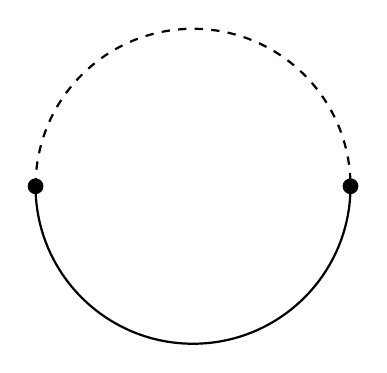
\begin{tikzpicture}
  \draw[thick] (0,2) arc(180:360:2);
  \draw[thick, dashed] (0,2) arc(180:0:2);
  \fill
    (0,2) circle (0.1)
    (4,2) circle (0.1)
  ;
\end{tikzpicture}
~~
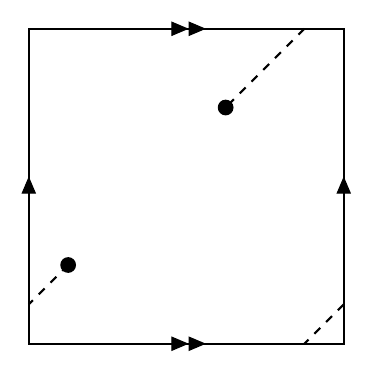
\begin{tikzpicture}
  \draw[thick] (0,0) rectangle (4,4);
  \draw[->>, >={triangle 45}] (0.25,0)--(2.25,0);
  \draw[->>, >={triangle 45}] (0.25,4)--(2.25,4);
  \draw[->, >={triangle 45}] (0,0.125)--(0,2.125);
  \draw[->, >={triangle 45}] (4,0.125)--(4,2.125);
  \fill
    (0.5,1) circle (0.1)
    (2.5,3) circle (0.1)
  ;
  \draw[thick, dashed]
    (0.5, 1)--(0,0.5) (4,0.5)--(3.5,0) (3.5,4)--(2.5, 3)
  ;
\end{tikzpicture}
    \caption{Illustrations of diameters on $S^1$ and $T^2$, and geodesics
    that achieve them.}
  \end{figure}

  \begin{theorem}[\cite{Liokumovich}]
    Let $M$ be a Riemannian $2$-sphere. Then there exist three distinct simple
    geodesics with lengths that do not exceed $20d$ where $d$ is the diameter
    of $M$.
    Furthermore, if no simple closed geodesics of length $\leq 2d$, then there
    are three distinct simple periodic geodesics on M with lengths
    $\leq 5d$, $10d$, \text{ and } $20d$ respectively.
  \end{theorem}
  \begin{proof}[Proof idea]
    The above authors give their proof idea as follows: \begin{quote}
      The main idea of the proof of [the above theorem] is to express three homology
      classes of the space of non-parametrized curves that are used in classical
      proofs of the Lyusternik-Schnirelmann theorem by cycles that consist of
      simple closed curves ``mainly made'' of curves in a meridian-like family
      that connects two fixed points of $M$. [...] We attempt to construct such
      a family where the lengths of all meridians are bounded by const d for an
      appropriate const. Our repeated attempts can be blocked only by appearance
      of different “short” simple periodic geodesics of index 0. So, we either
      get three short simple periodic geodesics of index 0, or our third attempt
      to construct a “meridional slicing” succeeds. Once one of our attempts
      succeeds, and we get a slicing of $M$ into short meridians, the original
      proof of the Lyusternik-Schnirelmann theorem yields the desired upper
      bounds.
    \end{quote}
  \end{proof}
  \begin{remark}
    With these bounds, it is natural to ask if all $2$-spheres have a fourth
    geodesic which has length bounded by the size of the manifold, but
    \cite{Liokumovich} writes:
    \begin{quote}
      [There is a] classical result of M. Morse, who proved that the fourth periodic
      [not necessarily simple] geodesic becomes uncontrollably large for
      ellipsoids with distinct but very close semi-axes.
    \end{quote}
  \end{remark}
\end{section}
\begin{section}{Conclusion}
  A quick final personal note: I find that the farther I get in my mathematical
  career, the deeper I have to dig to find new-to-me theorems that spark a
  sense of wonder, but I've found that this relatively simple topic is full
  of them, especially those discussed in the previous section.

  In particular, the theorem of three simple closed geodesics is quite
  unbelievable---especially when combined with the result that a fourth
  (perhaps non-simple) closed geodesic can be arbitrarily large. It's especially
  remarkable in the context of Conjecture 4.1, which says that it is not
  known whether or not simple closed geodesics exist on all compact manifolds.

  Thanks again for your help in suggesting this as a topic---I found the
  experience to be immensely rewarding.
\end{section}
% \begin{section}{Conclusion}
% \end{section}
\printbibliography
\end{document}
